\documentclass[dvipdfmx]{jarticle}
\usepackage{graphicx}
\usepackage[top=30truemm,bottom=30truemm,left=25truemm,right=25truemm]{geometry}
\usepackage{listings,jvlisting}
\usepackage{url}


\lstset{
  basicstyle={\ttfamily},
  identifierstyle={\small},
  commentstyle={\smallitshape},
  keywordstyle={\small\bfseries},
  ndkeywordstyle={\small},
  stringstyle={\small\ttfamily},
  frame={tb},
  breaklines=true,
  columns=[l]{fullflexible},
  numbers=left,
  xrightmargin=0zw,
  xleftmargin=3zw,
  numberstyle={\scriptsize},
  stepnumber=1,
  numbersep=1zw,
  lineskip=-0.5ex
}

\begin{document}
\begin{titlepage}
    \begin{center}
        {\huge 情報科学実験B 課題4レポ―ト}
        \vspace{180pt}\\
        \begin{tabular}{rl}
            氏名 & 山久保孝亮\\
            所属 & 大阪大学基礎工学部情報科学科ソフトウェア科学コース\\
            メールアドレス & u327468b@ecs.osaka-u.ac.jp\\
            学籍番号 & 09B22084\\
            提出日 & \today\\
            担当教員 & 松本真佑,小南大智
        \end{tabular}
    \end{center}
\end{titlepage}

\section{システムの仕様}
今回私が作成したのはブラウザ観賞用ジョイスティックマウスである.このマウスは,二つのジョイスティックを用いて実際のマウスの機能及びネットサーフィンをするうえで
便利な機能を追加したものである.以下にその機能を記述する.
\subsection{左手に持つジョイスティックの仕様}
\begin{enumerate}
    \item ジョイスティックを傾けることでマウスカーソルを移動させる.
    \item ジョイスティックを押し込むことで実際のマウスの右クリックと同じ結果になる.
\end{enumerate}
\subsection{右手に持つジョイスティックの仕様}
\begin{enumerate}
    \item ジョイスティックを上下に傾けることでホイール操作ができる.
    \item ジョイスティックを左に傾けることでブラウザ上での"戻る"ボタンを,右に傾けると"進む"ボタンを押したときと同じ結果となるようにした.
    \item ジョイスティックを押し込むことで実際のマウスの右クリックと同じ結果になる.
\end{enumerate}
\section{ハードウェア回路}
今回私が作成したハードウェア回路は以下の図1のようになる.\cite{1}\cite{6}
\begin{figure}[h]
    \centering
    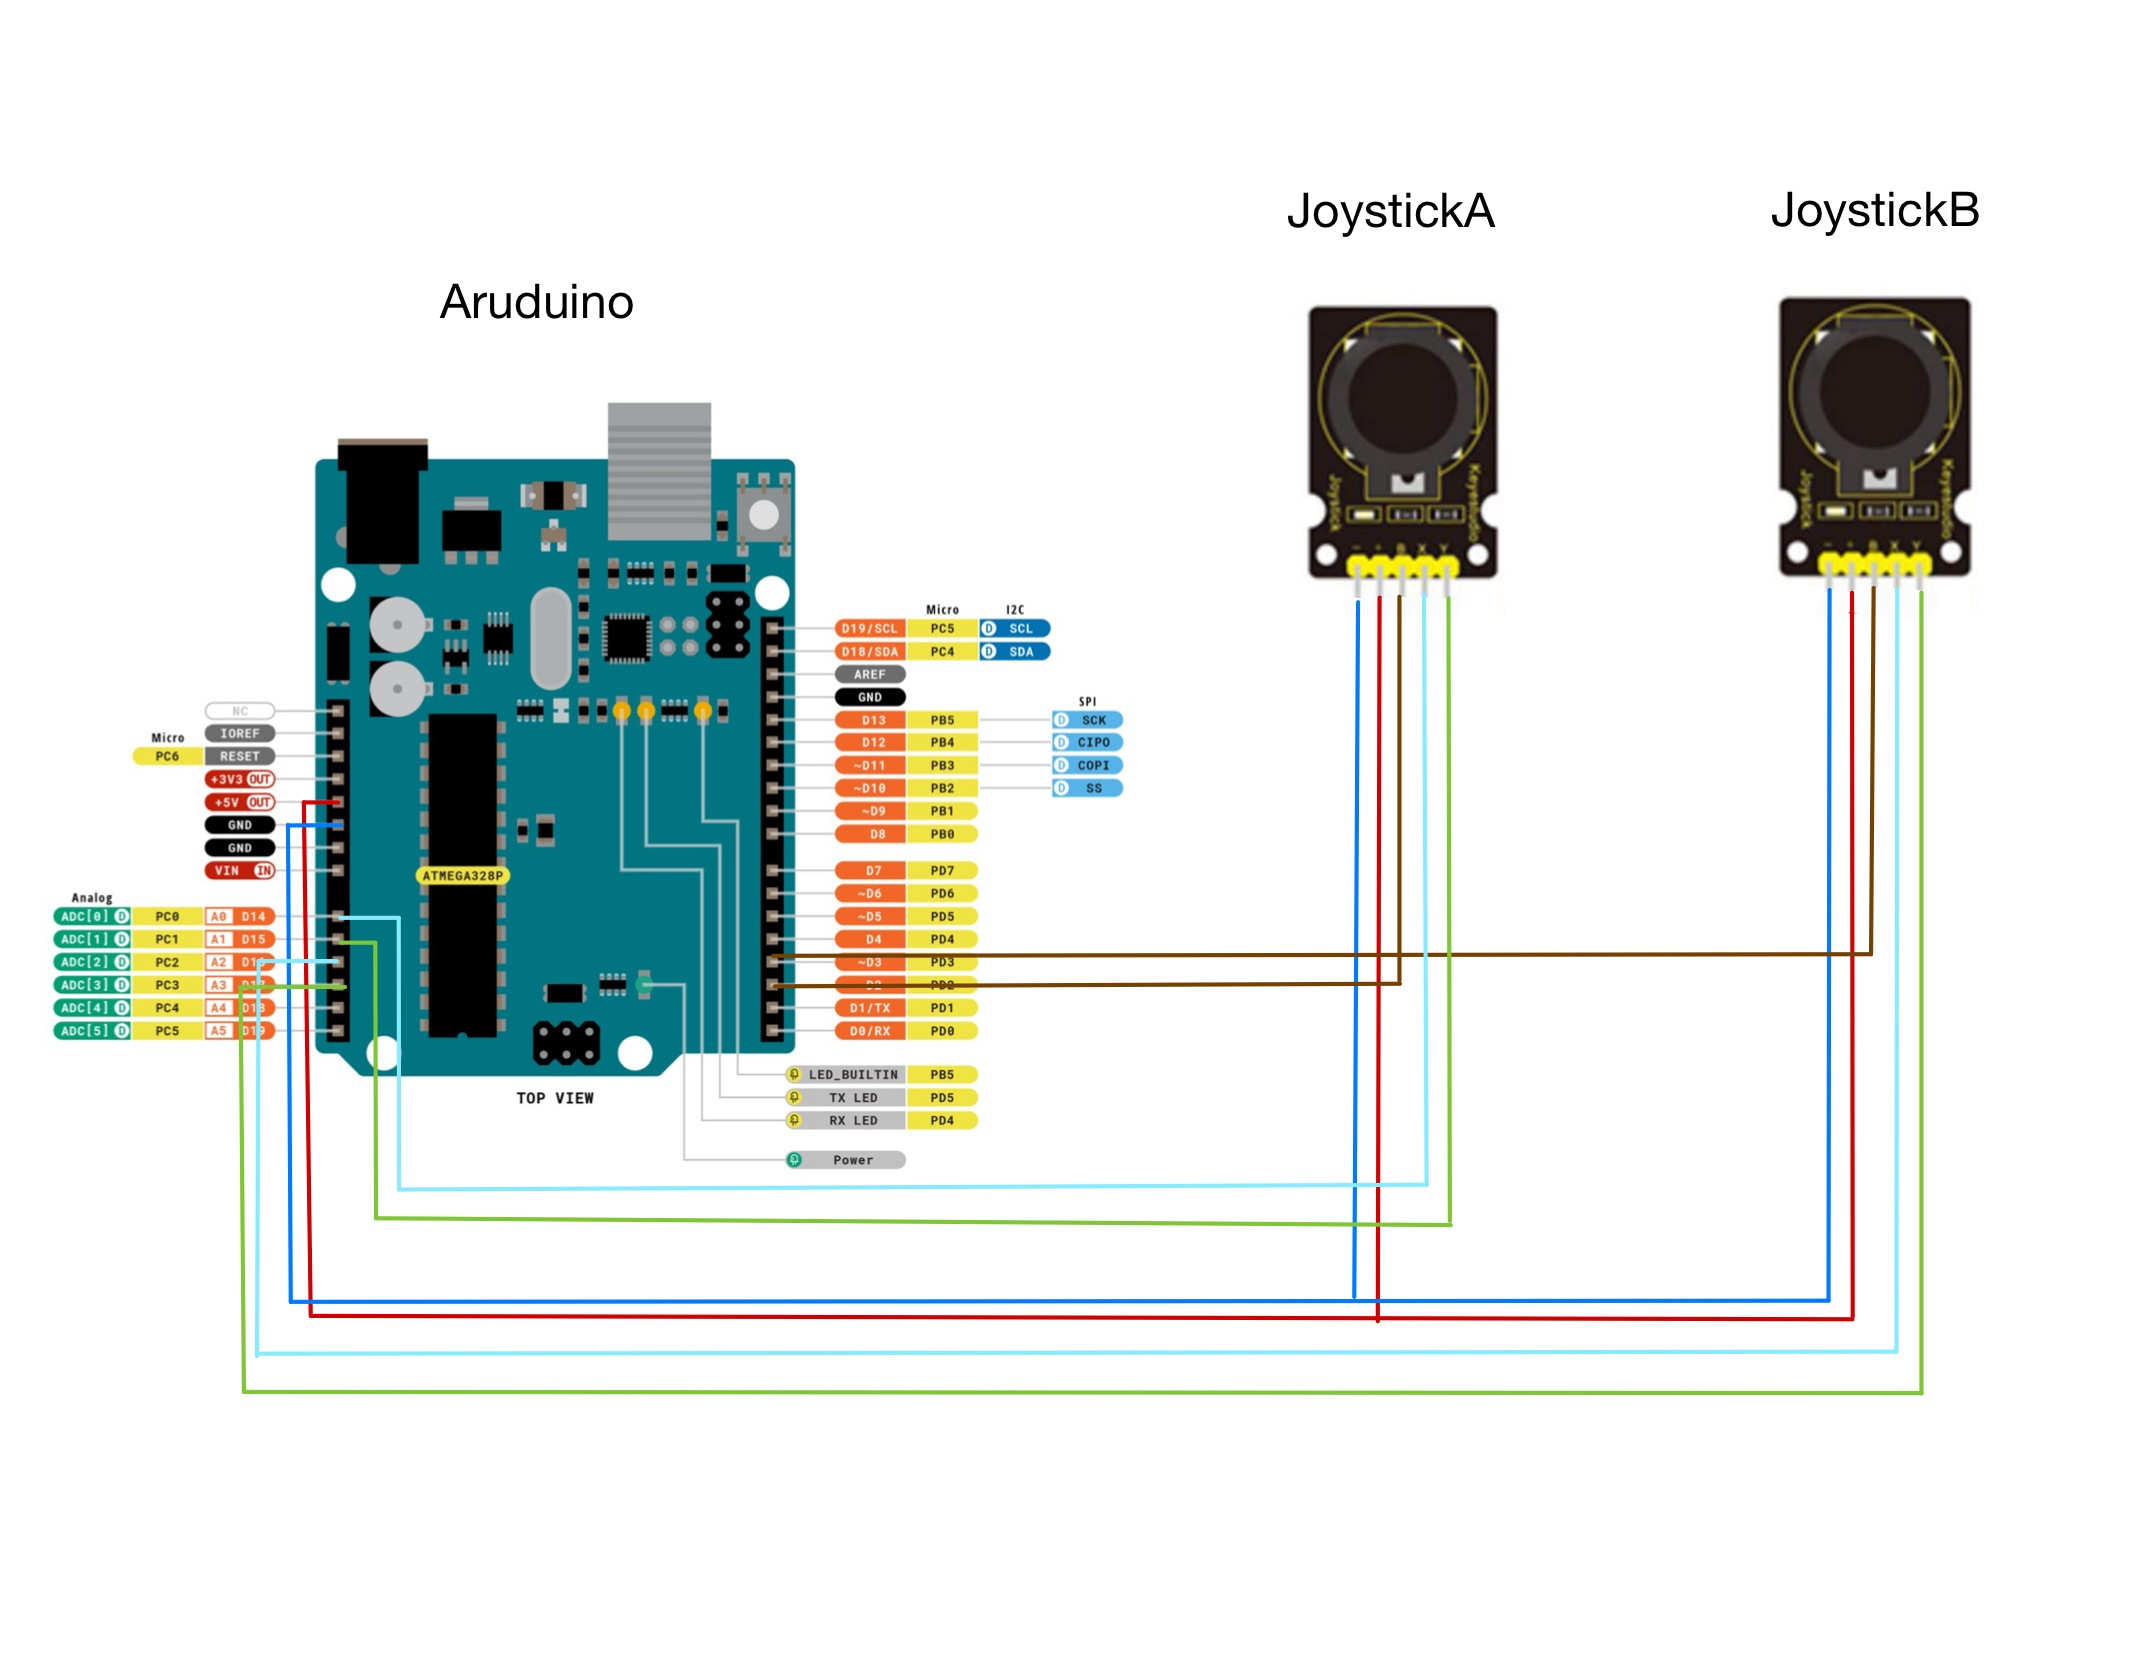
\includegraphics[width=8cm]{kairo.jpg}
    \caption{ハードウェア回路}
\end{figure}
\\ジョイスティックのピンは左から順番にグラウンド,5V,スイッチのピン,ジョイスティックの横方向の傾け度合い,ジョイスティックの縦方向の傾け度合いを
表すピンをそれぞれ接続する.今回は左手に持つジョイスティックAのスイッチのピンはD2に,右手に持つジョイスティックBのスイッチのピンはD3に設定した.
また,ジョイスティックAの傾け度合いは横方向と縦方向でそれぞれアナログピンA0とA1に,ジョイスティックBに関してはアナログピンA2とA3に設定した.
\\ここで,ジョイスティックの仕組みについて記述する.ジョイスティックは以下の図2のように,X軸,Y軸に対応した可変抵抗が存在する.\cite{7}
\begin{figure}[h]
    \centering
    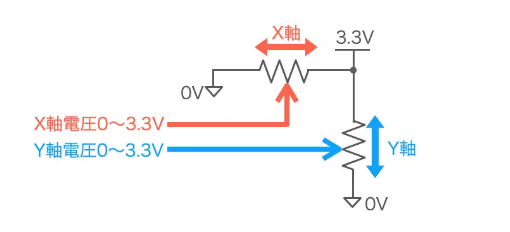
\includegraphics[width=8cm]{joystick.png}
    \caption{ジョイスティックの構造}
\end{figure}
\\これによりそれぞれの成分について0Vから3.3Vまでの値が出力され,スティックの操作位置を読み取ることができるようになる.
\section{制御プログラム}
今回のジョイスティックマウスを実現するに当たって,Arduino UnoではMouseライブラリを使用できなかったので
一旦シリアル通信でノートPCにジョイスティックから取得したデータを送信し,ノートPC内でPythonのプログラムを実行して
マウスに関する処理を実行した.\cite{2}したがって,今回のレポートの制御プログラムの説明ではジョイスティックから情報を取得しノートPCに送信するプログラム(Arduinoのプログラム)と,送られてきたデータからマウス
を操作するプログラム(Pythonのプログラム)に分けることができる.
\subsection{Arduinoのプログラム}
ここではArduinoのプログラムについて記述する.プログラムのフローチャートは以下のようになる.\cite{2}
\begin{figure}[h]
    \centering
    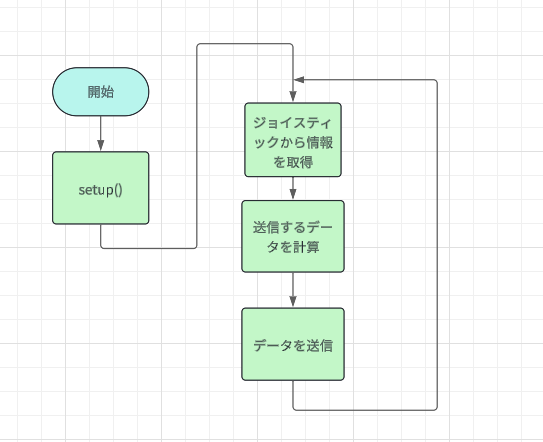
\includegraphics[width=8cm]{arduino_huroty.png}
    \caption{Arduinoのプログラムのフローチャート}
\end{figure}
このフローチャートに基づいてプログラムを説明する.まず,今回使用したピンの情報は以下のようになる.
\begin{lstlisting}
const int xPinA = A0;
const int yPinA = A1;
const int xPinB = A2;
const int yPinB = A3;
const int buttonPinA = 2;
const int buttonPinB = 3;
\end{lstlisting}
A0とA1はそれぞれ左手側のジョイスティックのx軸,y軸のピン,A2とA3は右手側のジョイスティックのx軸,y軸のピンを表す.
buttonPinAは左手側のジョイスティックを押し込んだ時のピンを,buttonPinBは右手側のジョイスティックを押し込んだ時のピンを表す.
\subsubsection{setup()の処理}
setup()ではシリアル通信を開始し,それぞれのピンモードを指定する.
\subsubsection{ジョイスティックから情報を取得}
これ以降の記述はloop()内の処理である.ここではまずジョイスティックから情報を取得する.そのためのコードは以下のようになる.
\begin{lstlisting}
int xValueA = analogRead(xPinA);
\end{lstlisting}
analogRead()は引数にピン番号を入れると返り値として0から1023までの整数値を返す.これをxPinB,yPinA\\
,yPinBにも使用してジョイスティックから情報を取得し,xValueB,yValueA,yValueBに格納する.また,digitalRead()を使用してボタンの状況も情報を取得する.
\subsubsection{送信する情報を計算}
次に,送信する前の段階である程度データを計算しておく.
ここで計算するデータは以下の通りである.
\begin{lstlisting}
int A_X_Vector = 0, A_Y_Vector = 0, B_X_Vector = 0, B_Y_Vector = 0;
\end{lstlisting}
Aを含む変数はマウスカーソル,Bを含む変数はホイールや進む,戻るボタン等に対応している.
ここで0に初期化をしているのは,ジョイスティックのわずかな変化によってマウスカーソル及びホイールが変化しないようにするためである.詳細はのちに記述する.
次に,以下のような条件分岐を上で初期化した4つの変数に対して行う.
\begin{lstlisting}
if (xValueA >= 550) {
    A_X_Vector = map(xValueA, 550, 1023, 0, sensitivity);
} else if (xValueA <= 450) {
    A_X_Vector = map(xValueA, 450, 0, 0, -sensitivity);
}
\end{lstlisting}
これは,xValueの値が450から550までの間はどちらの条件分岐にも入らないようになっている.450と550を境界値にした理由としては,analogRead()による結果が0から1024であり,中央値が約500であることからそこからそれぞれ50ずつをジョイスティックの変化として考えないようにしたためである.このときはA\_X\_Vectorの値が
初期値の0のままとなる.これによってジョイスティックのわずかな変化には反応しないようになっている.
xValueの値が550以上の場合はmap()を使用してA\_X\_Vectorの値を変更している.map()は第二引数から第三引数までしかとらない第一引数の値を,第四引数から第五引数の間の値に変更する関数である.\cite{4}

また,sensitivityは変更後の最大値であるから,この値を変更することでマウスカーソル等の感度を変更することができる.デフォルトでは10とした.
\subsubsection{データの送信}
今回のプログラムでは以下のようにデータを","で区切って送信した.
\begin{lstlisting}
Serial.print(A_X_Vector);
Serial.print(",");
Serial.print(A_Y_Vector);
Serial.print(",");
Serial.print(B_X_Vector);
Serial.print(",");
Serial.print(B_Y_Vector);
Serial.print(",");
Serial.print(buttonStateA == LOW ? 1 : 0); 
Serial.print(",");
Serial.println(buttonStateB == LOW ? 1 : 0);
\end{lstlisting}
9行目と11行目のbuttonStateに関しては,それぞれボタンが押されていれば0を,ボタンが押されていなければ1を送信する.
\subsection{Pythonのプログラム}
ここではPythonのプログラムについて記述する.プログラムのフローチャートは以下のようになる.
\begin{figure}[h]
    \centering
    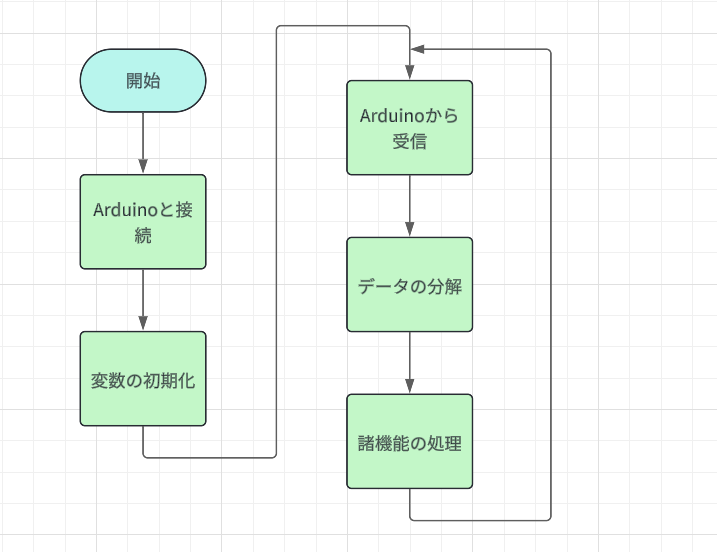
\includegraphics[width=8cm]{python_hurotya.png}
    \caption{Pythonのプログラムのフローチャート}
\end{figure}
このフローチャートに基づいてプログラムを説明する.
\subsubsection{Arduinoと接続}
以下のようなプログラムでArduinoとPCを接続した.
\begin{lstlisting}
ArduinoSerial = serial.Serial('COM3',9600)
time.sleep(1)
\end{lstlisting}
2行目はArduinoとの接続を安定させるためである.
\subsubsection{変数の初期化}
次に変数を初期化する.
\begin{lstlisting}
back_interval = 1
last_back_time = 0
forward_interval = 1
last_forward_time = 0
previous_right_button = 1
previous_left_button = 1
\end{lstlisting}
1から3行目は"戻る"機能を,4から6行目は"進む"機能を実現するための変数であり,フローチャートの繰り返しが始まる前に
初期化している.
\subsubsection{Arduinoから受信}
フローチャートのように,以下で記述する内容は無限ループの中の処理である.接続されたArduinoから送られてきたデータを取り出す操作は以下のプログラムで実現される.
\begin{lstlisting}
data = ArduinoSerial.readline().decode('utf-8').rstrip()
values = data.split(",")
if len(values) != 6:
    print(f"Unexpected data format: {data}")
    continue
\end{lstlisting}
まずdataに送られてきたUTF-8の文字列から改行文字を取り除いたものを格納する.
そのdataはArduinoのプログラムで記述したように","で区切られているので2行目のsplit()を使って分け,リストとなりvaluesに格納される.
リストvaluesの長さが想定している6でなければ,条件分岐させエラーメッセージとともに繰り返しの最初まで戻す.この処理の目的は,期待された受信データとは異なる形式として
受け取ったデータを使用してマウスの処理をしてしまうことを避けるためである.期待されたデータの形式であれば,continue以下のプログラムが処理される.
\subsubsection{データの分解}
データの分解は以下のプログラムによって行われる.
\begin{lstlisting}
left_x_vector, left_y_vector ,right_x_vector ,right_y_vector ,left_button ,right_button = map(int , data.split(","))
\end{lstlisting}
map()を使って各要素をint型に変更しそれぞれの変数に格納する.それぞれの変数については3.2.5の諸機能の処理にて詳細を記述する.
\subsubsection{諸機能の処理}
ここでは今回実現したマウス操作に関する様々な機能の実現方法を記述する.\\
まずはマウスカーソルの操作について記述する.
\begin{lstlisting}
(mouse_x,mouse_y) = mouse.get_position()
mouse.move(mouse_x+left_x_vector,mouse_y-left_y_vector)
\end{lstlisting}
上のプログラムの一行目では現在のマウスカーソルのx座標とy座標をget\_position()を使用して取得している.そしてそれらに3.2.4で取得した
左手に持つジョイスティックから得られる,どれだけマウスカーソルを移動させるかを表すleft\_x\_vectorとright\_y\_vectorを合わせたものを引数としてmove()を使って移動させる.
ここで縦軸に関して加算ではなく引き算をした理由は,縦軸の正の方向が画面の下側であるためである.\cite{5}\\
次に記述するのはそれぞれのジョイスティックを押し込んだ時の機能である.
\begin{lstlisting}
if right_button == 0 and previous_right_button == 1:
    mouse.click('left')
if left_button == 0 and previous_left_button == 1:
    mouse.click('right')
---------------------------------------------------------------------------------
previous_right_button = right_button
previous_left_button = left_button
\end{lstlisting}
1行目と3行目の条件文は,それぞれのジョイスティックが押し込まれたタイミングかどうかを判定している.
それぞれが押し込まれた瞬間にmouse.click()を使って左クリックと右クリックの機能を実現している.右手のジョイスティックを押したときに左クリック,左手のジョイスティック
を押したときに右クリックのように,実際のマウスと左右を反転させた理由としてはジョイスティックを操作しながら押し込むという操作が難しいと感じたためである.また,点線以下の6,7行目は繰り返しの最後に
現在のボタンの状態を記憶するものであり,条件分岐の際に使用される.\\
次にホイール操作について記述する.
\begin{lstlisting}
if right_y_vector != 0:
    wheel_speed = np.interp(right_y_vector,(-10,10),(-1,1))
    mouse.wheel(wheel_speed)
\end{lstlisting}
右手側のジョイスティックの縦方向の傾け度合いを格納しているright\_y\_vectorが0でなければ,
np.interp()を使って-1から1の値になるように値を変更しホイール操作の速度を計算する.そしてmouse.wheel()を使用してホイール操作を行う.
mouse.wheel()の引数には-1から1の値までしか取れないために速度を計算した.\\
最後に"戻る"機能と"進む"機能の処理について記述する.
\begin{lstlisting}
if right_x_vector < -5:
    current_back_time = time.time()
    if current_back_time - last_back_time >= back_interval:
        pyautogui.hotkey('alt', 'left')
        last_back_time = current_back_time
if right_x_vector > 5:
    current_forward_time = time.time()
    if current_forward_time - last_forward_time >= forward_interval:
        pyautogui.hotkey('alt', 'right')
        last_forward_time = current_forward_time
\end{lstlisting}
右手側のジョイスティックの横方向の方向け度合いを格納しているright\_x\_vectorの値はArduinoのプログラムで示したように,-sensitivityからsensitivityの値まで取ることができる.
今回はsensitivityが10であるときの処理である.戻る機能や進む機能は少しの変化で反応してしまうと間違えてその操作をしてしまう可能性がある.したがって,
sensitivityの半分の値になるまでジョイスティックを傾けないと処理されないように設定した.
\section{考察や工夫点}
今回の課題を通して私が考察したのはマウスやトラックボール等ではなくジョイスティックを使用することの是非ついてである.\\
今回のジョイスティックマウスが先ほど挙げたマウスなどと異なる点は机などの平面に接地していなくてもよいという点である.トラックボールマウス等はどの場所に置いても操作することはできるが安定した場所でないと本来の操作感は得られない.
ジョイスティックなら手を机からおろしたような場所であっても操作することが可能である.今回作成したものはArduinoに接続されているためジョイスティックを動かす範囲が制限されてしまっているが,
Bluetooth等を用いてジョイスティックの情報を離れたところから伝達できるようになれば自由に持ち運べるようにできると考えられる.このジョイスティックマウスの効果的な使用方法としてはパソコンの画面をテレビ等に映して動画や映画を鑑賞する際に使用できる点だと私は考えた.
これは,リモコンよりもマウスの操作性に近くなるためである.

しかし,マウスカーソルの操作感などについては改良の余地があると感じたのでsensitivityやジョイスティックのどのあたりまで反応しないようにするか等の調整などが課題としてあげられる.
\section{感想}
今回の課題を通して私が感じたことは自分で考えることの楽しさである.これまでの実験やプログラミングの授業では指定された仕様を満たすような課題を作成してきたが,
実験Bの課題4に関しては何を作るのかが生徒側に委ねられていた.最初は何を作るべきが迷ってしまい時間を持て余していたが一度方向性が固まるとどんな機能を追加すればよいかなどを考えることに
楽しみを見出すことができた.4回生や大学院に進学した後に行う研究も私が何をするのかを決めることになるので,今回の課題での経験は非常に役立つものになると感じた.
\section{謝辞}
4月から約4か月間授業中の質問対応やレポート採点などをしてくださった教授,TAの皆様,本当に有難うございました.この授業で学んだことを活かして,
今後の学習及び研究に取り組んでいきたいと思います.
\begin{thebibliography}{99}
    \bibitem{1} \url{https://docs.keyestudio.com/projects/KS0349/en/latest/KS0349.html#project-36-joystick} 7/11アクセス
    \bibitem{2} \url{https://elchika.com/article/137e8fc6-cc28-420e-b41d-d75da29f6568/} 7/11アクセス
    \bibitem{3} \url{http://www.musashinodenpa.com/arduino/ref/index.php?f=0&pos=2113} 7/11アクセス
    \bibitem{4} \url{http://www.musashinodenpa.com/arduino/ref/index.php?f=0&pos=2743} 7/11アクセス
    \bibitem{5} \url{https://laboratory.kazuuu.net/using-mouse-to-control-a-mouse-in-python/} 7/16アクセス
    \bibitem{6} 情報科学実験B指導書
    \bibitem{7} \url{https://logikara.blog/joystick/} 7/20アクセス
\end{thebibliography}
\end{document}